% SLOGAN: How to know when you don't have a kind.
% Sticky sentence: "Not every stable pattern is a homeostatic cluster."

\chapter{Failure modes}
\label{ch:failure-modes}


The danger of a good framework is that you start seeing it everywhere.

Once you learn to spot homeostatic property clusters~-- once you see how feedback loops can maintain stable patterns without essences~-- it becomes tempting to diagnose homeostasis in every corner of the grammar. \term{Noun}? HPC. \term{Subject}? HPC. \term{Voice}? HPC. \term{Non-finite}? Surely an HPC too. The world fills up with spinning tops.

This is the \term{inflation problem}. If the criteria for being a mechanism-maintained kind are too loose, the framework explains nothing because it excludes nothing. If every stable pattern counts as an HPC, then \enquote{HPC} just means \enquote{pattern we have a name for.}

But not every top is the same. Some wobble for a moment and fall; some were never really spinning~-- just labels we applied to patterns that happened to be there. Section~\ref{sec:4:heterogeneity} previewed three ways a category can miss: thin, fat, or negative. This chapter develops the diagnostics. The answer turns out to be that the ways a category can miss tell us something about what it takes to be a genuine kind.

\section{The inflation problem}
\label{sec:8:inflation}

Why are some categories so tempting to reify? Why does linguistics~-- and cognition generally~-- generate labels that feel like kinds but turn out to be something else?

Start with a familiar example. What makes something a \term{chair}? In terms of physical properties~-- materials, shape, construction~-- a bean bag, a papasan, a recliner, and a three-legged Frank Lloyd Wright design have almost nothing in common. But from the perspective of someone who wants to sit down, they're all the same. The category \term{chair} groups objects by what they do for us, not by what they are.

This is a useful category. If you know something is a chair, you know you can sit on it. But is it a \emph{natural kind}? Are there mechanisms maintaining \enquote{chairness} as a stable cluster of properties in the objects themselves? No~-- individual bean bags and recliners are manufactured by independent causal chains. The category tracks \emph{function}, not underlying structure~-- and this isn't the \enquote{functional pressure} that §\ref{sec:7:stabilisers-at-scales} identifies as a stabiliser; that applies when function shapes what gets transmitted, not when function is merely the criterion by which a user groups pre-existing objects. (Word-kinds are different: \mention{chair} as a lexeme \emph{is} maintained by mechanisms~-- entrenchment, alignment, transmission~-- but the category of objects it refers to is not.)

The same logic applies to \term{dessert}, \term{trash}, \term{weapon}. These categories are useful for making decisions. Knowing something is a weapon tells you to be cautious. But the usefulness comes from how they fit into our activities, not from shared mechanisms that maintain them as kinds. (Individual sub-categories~-- \term{gun}, \term{sword}, \term{croissant}~-- may well have their own transmission lineages; the claim is that the umbrella grouping \term{weapon} or \term{dessert} lacks a unifying mechanism across its heterogeneous members.) Khalidi calls such categories \term{epistemic kinds}: they serve our epistemic purposes~-- classification, description, prediction~-- but don't necessarily track causal structure in the world \autocite[43, 65]{khalidi2013}.

Now translate to linguistics. The analyst's job is to describe language. Categories earn their keep by making description tractable. If grouping manner adverbs, degree words, and sentence adverbs under a single label \term{adverb} simplifies the grammar, the label is useful~-- even if no mechanism unites those items.

The inflation problem arises when we mistake this usefulness for reality. We see that \term{adverb} is useful~-- it tells us \enquote{this modifies something other than a noun}~-- and we assume there must be a deep, unified mechanism maintaining all adverbs as a natural kind. We confuse the utility of the label with the reality of the cluster. (The philosopher Cailin O'Connor has formalised this insight using evolutionary game theory, showing how categories optimised for coordination can diverge from categories that track real structure; see \citealt{oconnor2019games}.)

The inflation problem is compounded by \emph{material reinforcement}. Some labels don't just circulate in heads; they circulate in curricula, exams, style guides, tagsets, and parsers. When a category is institutionally scaffolded~-- taught in schools, encoded in annotation standards, rewarded by grading rubrics~-- it can look stable and projectible even if the underlying mechanisms are weak or absent. Stability is not enough. A category with no real mechanistic basis can persist for centuries if institutions reward it.

Here's the trap: categories can be useful, learnable, stable across generations~-- and still fail to be natural kinds. The question this chapter addresses is how to tell the difference: when does an epistemic kind also pick out a genuine HPC, and when is it merely a convenient label?



\section{The two diagnostics}
\label{sec:8:diagnostics}

To answer that question, we need criteria. Chapter~\ref{ch:projectibility} argued that projectibility is the epistemic payoff of genuine kinds: a category earns its keep by supporting induction. Chapter~\ref{ch:stabilisers} argued that homeostasis is the ontological ground: a category is real because mechanisms maintain it. These two faces of the HPC definition give us two diagnostics. To warrant the claim that a linguistic category is an HPC kind, it must pass both.

\subsection{The projectibility diagnostic}
\label{sec:8:projectibility-diagnostic}

\emph{Can we predict new data from old?}

If a category is a genuine kind, learning its properties from a finite sample should allow you to predict unobserved instances. This is projectibility: the pattern travels. In §\ref{sec:6:definitional-bet}'s terms, it's the \emph{good bet}~-- you stake what you've learned and the bet pays off.

The test is straightforward. Train a model~-- or a learner~-- on one dataset: a corpus, a time period, a set of languages. Test on a held-out set. If performance significantly exceeds baseline (e.g., shuffled labels), the bet was good; the pattern is projectible. If the model overfits or collapses on new data, the bet was bad; the pattern is local, accidental, or illusory. Shuffled labels are the lie detector for category romance.

Polish aspect offers the worked example (§\ref{sec:6:definitional-bet}). The textbook semantic definitions~-- boundedness, totality~-- project imperfective well (98\%) but perfective poorly (77\%). The definitional bet fails for half the system. By contrast, the lemma-concrete model~-- which learns cue--outcome associations without representing aspect as a category~-- projects better across the board. Good bets track mechanisms, not labels.

A confound lurks here. Projectibility across corpora can be an artefact of shared conventions~-- genre pipelines, annotation guidelines, register selection, editorial norms~-- rather than evidence of genuine mechanistic clustering. A category that predicts well across the British National Corpus, the Corpus of Contemporary American English, and the Penn Treebank may do so because all three were annotated by linguists trained in the same tradition, not because the category tracks stable structure in ordinary speech. This is why the two-diagnostic test is necessary: the homeostasis diagnostic (perturbation sensitivity) guards against convention-driven projectibility.

\subsection{The homeostasis diagnostic}
\label{sec:8:homeostasis-diagnostic}

\emph{Can we name the stabilisers?}

If a category is a genuine kind, its stability must be causal, not accidental. We should be able to identify the specific feedback loops maintaining it: acquisition, entrenchment, alignment, transmission, functional pressure.

The test asks: can we trace the causal chain? Can we predict what would happen if a stabiliser were removed? A genuine HPC should exhibit perturbation-sensitivity: weaken a mechanism, and the cluster should fray. A mere label should be perturbation-inert: remove it, and nothing changes in production or acquisition. This operationalises the homeostasis criterion in ways philosophers have demanded: \textcite{craver2009} argued that HPC theory is vague about what counts as a mechanism and where one mechanism ends and another begins. The perturbation test provides a concrete answer: we recognise a mechanism by countering it~-- whatever process, when weakened, causes the cluster to fray. This is a diagnostic criterion, not a definition; it tells us how to find mechanisms, not what they essentially are.

This diagnostic catches categories that are projectible by accident. A local correlation might predict well within a corpus but lack any causal grounding. The homeostasis diagnostic asks: is there a feedback loop, or just a coincidence?

Heritage language attrition provides a natural experiment. When transmission mechanisms weaken~-- when children receive reduced input because their parents speak the heritage language less, or when community alignment is diluted by a dominant contact language~-- category boundaries become variable in predictable ways. Polinsky's work on American Russian shows exactly this pattern: heritage speakers maintain high-frequency, highly entrenched items (core vocabulary, basic constructions) while low-frequency items drift or are replaced by contact-language calques \autocite{polinsky2018heritage}. The perturbation (reduced transmission) causes the cluster to erode at its margins while the core holds. This is what the homeostasis diagnostic predicts: genuine HPCs show perturbation-sensitivity, with the degree of drift proportional to the strength of the perturbed mechanism.

\subsection{Why both are needed}

A category can pass one diagnostic and fail the other.

A category might be projectible but not homeostatic. Consider a corpus artifact~-- a distributional pattern that emerges from a particular text genre or register. Within that corpus, the pattern predicts well. But there's no mechanism maintaining it; shift to a different corpus, and it vanishes. The projectibility was real but local; the homeostasis was illusory.

A category might be homeostatic but not projectible. Consider a category maintained by a single, weak mechanism that operates inconsistently across speakers. The mechanism is real~-- we can name it, intervene on it~-- but it doesn't produce enough clustering to support reliable prediction. The homeostasis is real but insufficient.

Categories that pass both diagnostics are good candidates for HPC status. Categories that fail one or both are suspect. The three failure modes we'll examine each fail in characteristic ways:

\begin{itemize}
    \item \textbf{Thin classes} miss the homeostasis diagnostic. The mechanisms are absent or too weak to produce stable clustering.
    \item \textbf{Fat classes} miss the projectibility diagnostic. The label lumps distinct mechanisms, so learning one subclass doesn't generalise to others.
    \item \textbf{Negative classes} miss both. They're defined by absence, with no positive property cluster to maintain or project from.
\end{itemize}

\begin{table}[t]
\centering
\caption{Failure modes of putative HPC kinds}
\label{tab:failure-modes}
\begin{tabular}{@{}llll@{}}
\toprule
\textbf{Failure mode} & \textbf{Projectibility} & \textbf{Homeostasis} & \textbf{Example} \\
\midrule
Thin & Fail (insufficient clustering) & Fail (no stabilisers) & Preposition doubling \\
Fat & Fail (subclass divergence) & Partial (subgroup mechanisms) & Umbrella \term{adverb} \\
Negative & Fail (no positive cluster) & Fail (defined by absence) & \term{Non-finite} \\
\bottomrule
\end{tabular}
\end{table}

\begin{figure}[t]
\centering
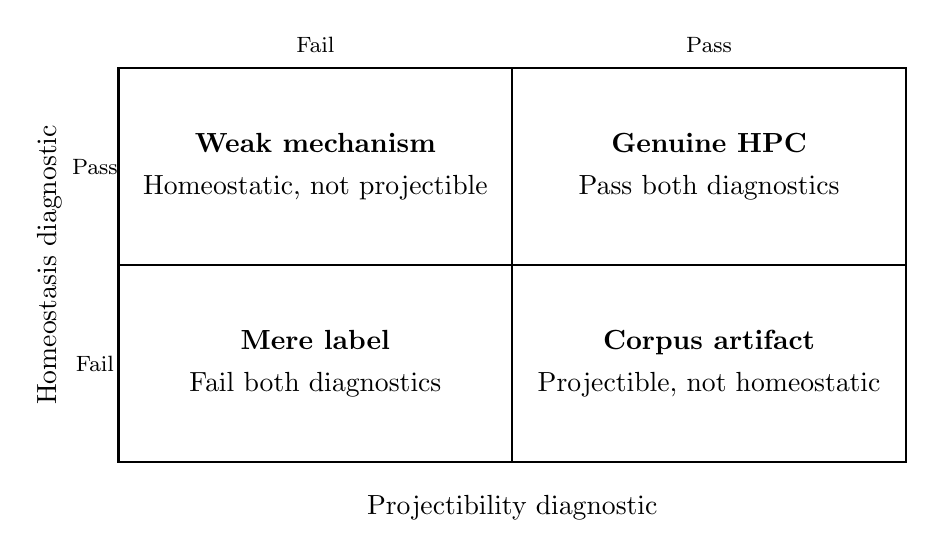
\begin{tikzpicture}[
    box/.style={rectangle, draw, minimum width=5cm, minimum height=2.5cm, align=center, font=\small},
    label/.style={font=\footnotesize\itshape}
]
% Grid
\draw[thick] (0,0) -- (10,0) -- (10,5) -- (0,5) -- cycle;
\draw[thick] (5,0) -- (5,5);
\draw[thick] (0,2.5) -- (10,2.5);

% Quadrant labels (simplified)
\node[align=center] at (2.5,3.75) {\textbf{Weak mechanism}\\[3pt]Homeostatic, not projectible};
\node[align=center] at (7.5,3.75) {\textbf{Genuine HPC}\\[3pt]Pass both diagnostics};
\node[align=center] at (2.5,1.25) {\textbf{Mere label}\\[3pt]Fail both diagnostics};
\node[align=center] at (7.5,1.25) {\textbf{Corpus artifact}\\[3pt]Projectible, not homeostatic};

% Axis labels
\node[rotate=90, anchor=south] at (-0.6,2.5) {Homeostasis diagnostic};
\node[anchor=north] at (5,-0.3) {Projectibility diagnostic};
\node at (2.5,5.3) {\footnotesize Fail};
\node at (7.5,5.3) {\footnotesize Pass};
\node at (-0.3,3.75) {\footnotesize Pass};
\node at (-0.3,1.25) {\footnotesize Fail};
\end{tikzpicture}
\caption{The two-diagnostic matrix. Only categories in the upper-right quadrant are genuine HPC kinds. Examples: \emph{Genuine HPC}~-- count noun, manner adverb; \emph{Weak mechanism}~-- idiolectal patterns; \emph{Mere label}~-- \term{non-finite}, umbrella \term{adverb}; \emph{Corpus artifact}~-- genre-specific patterns.}
\label{fig:diagnostic-matrix}
\end{figure}

\subsection{The grain question}

One more trap before the case studies: the problem of grain. Even when we have genuine HPCs, we often group them into larger systems labelled \enquote{Grammar} or \enquote{Language.} Is \term{English Morphosyntax} an HPC kind?

The temptation is to say yes. It's stable, it's learned, it's maintained. But this is the \term{Madagascar fallacy}. Biological species are the paradigmatic HPC kinds. \textit{Lemur catta} (the ring-tailed lemur) is a homeostatic cluster maintained by interbreeding, shared ecology, and genetic transmission. But consider \enquote{the fauna of Madagascar.} It is a stable collection of animals. It is distinct from the fauna of Australia. It has a causal history (isolation). But \enquote{the fauna of Madagascar} is not itself a species. It is an \emph{ecosystem} of species. There is no single mechanism that maintains \enquote{the fauna} as a unit; there are thousands of mechanisms maintaining the individual populations that comprise it. The fauna of Madagascar is not a species; it's an airline route plus a geological history.

Language is an ecosystem. The HPCs are the components~-- constructions, lexemes, phoneme contrasts, sometimes families or paradigms~-- not the grammar as a whole. The failure modes below apply at that level: we ask whether \term{adverb} is a kind, not whether \term{English} is. Section~\ref{sec:8:grain} returns to this question; for now, the point is that grain matters. A category can be too thin, too fat, too negative~-- or simply at the wrong level of analysis.


\section{Thin clustering: The smoke ring}
\label{sec:8:thin}

The first pattern is the category that barely exists.

A \term{thin} class is one where the signal exists~-- speakers recognise it, linguists name it~-- but the property cluster is ghostly. There is no robust homeostatic loop maintaining it. It's a \enquote{smoke ring}: it has structure, but that structure is ephemeral, typically generated by a transient convergence of other mechanisms rather than a dedicated feedback loop of its own.

Thin classes miss the homeostasis diagnostic. We can't name their stabilisers~-- because there are none, or none sufficient to produce stable clustering.

\subsection{The nonce word test}

\citet[25--26]{miller2021} provides a useful operationalisation. Whether a novel form counts as a \enquote{word-kind} depends on whether stabilising mechanisms~-- internal (cognitive) and external (social)~-- have emerged to maintain it as more than a one-off performance. Consider \term{cromulent}, coined for a 1996 \emph{Simpsons} episode to mean \enquote{acceptable, fine.}

Does \term{cromulent} exist as a word? Miller's answer is to treat this as a mechanistic question, not a metaphysical one. Are there internal routines ensuring that speakers reproduce the form reliably (phonology, meaning, inflectional behaviour)? Are there external norms that support convergent use (shared recognition, uptake, correction, expectation)? Within Simpsons-fan communities, the answer is often yes: the form is used with a consistent meaning and a stable pronunciation, and it is recognisable enough to support coordination. Outside those communities, the mechanisms are weaker or absent: the form surfaces as an in-joke, may be misheard or reanalysed, and is rarely transmitted as a general-purpose lexical item.

The point is not that \term{cromulent} is \enquote{real} for some speakers and \enquote{fake} for others, but that wordhood is a claim about where stabilisers are doing work. A form can be a bona fide HPC kind in one network and a thin pattern in another. The question is always: what maintains it, and at what scale?

The nonce word test generalises. A category is thin when the stabilisers that would make it a good bet have not (yet) consolidated. This can happen for genuinely new items (nonce coinages), for rare or enclave-restricted items (idiolectal or micro-community vocabulary), or for patterns that persist only as incidental fallout from other, more robust systems.

\subsection{Case study: Preposition copying and pruning}

English offers two options for relativising prepositional complements: pied-piping (\mention{the box in which I put it}) and stranding (\mention{the box which I put it in}). Both are robustly maintained. But at very low frequency, speakers produce outputs that either copy the preposition or omit it:

\begin{quote}
\textbf{Copying:} \mention{from which to choose from}, \mention{from where it came from}\\
\textbf{Pruning:} \mention{That's the situation that Obama finds himself} (intended: \mention{finds himself in})
\end{quote}

This pattern exists, and \citet{radford2012} document it in live broadcast speech: roughly 15 copying tokens and 67 pruning tokens in \textasciitilde300 hours of recording. Such forms often pass without overt repair, so the pattern is reproducible~-- but it is thin.

The frequency is vanishing~-- too rare to be plausibly acquired as a \emph{target} construction~-- and there's no social indexing (copying/pruning signals nothing about identity, register, or stance) or functional niche (either pied-piping or stranding serves the same communicative end without redundancy or omission).

Apply the homeostasis diagnostic: can we name the stabilisers?

\begin{itemize}
    \item \textbf{Acquisition:} Weak. The token rate is too low for learners to extract a dedicated rule.
    \item \textbf{Entrenchment:} Weak. No speaker uses it frequently enough for strengthening at the constructional level.
    \item \textbf{Social indexing:} Absent. There is no community norm that rewards or recognises it.
    \item \textbf{Functional pressure:} Absent. Competitors cover the function without any gap.
\end{itemize}

What generates copying and pruning is not a dedicated maintenance loop but online production under competition. Radford and Felser analyse these as performance-side phenomena: speakers begin constructing one option and drift toward the other midstream. In copying, the two options leave traces of both routes; in pruning, the preposition is lost under the same competitive pressure plus ordinary omission. Either way, the result is a byproduct of mechanisms that robustly maintain pied-piping and stranding, not a target of maintenance in its own right.

Compare to robust stranding: \mention{Who did you talk to?} This form is maintained by every mechanism on the list~-- frequency is high, it's acquired early, and it participates in register contrasts with pied-piping that create genuine indexical structure. Functional load is substantial. Preposition stranding is an HPC; copying/pruning is its smoke ring~-- cast off by the same dynamics but lacking the immune system to persist independently.

The perturbation test makes this vivid. If English lost preposition copying tomorrow~-- if speakers simply stopped producing it~-- no feedback loop would kick in to restore it. No acquisition pressure, no social correction, no functional gap. It would vanish without a trace. A genuine HPC resists perturbation; a smoke ring dissipates.

Robust HPCs are attractors: the mechanisms pull deviant instances back toward the cluster. Thin patterns are metastable: they persist only so long as the surrounding system continues to generate them as incidental fallout. This is what it means to fail the homeostasis diagnostic. The pattern is real~-- it can be observed, described, named~-- but the causal structure that would maintain it is absent. We have a label without a kind.

\section{Fat clustering: The wastebasket}
\label{sec:8:fat}

The second pattern is the opposite of thinness: not too little mechanism, but too many pulling in different directions.

A \term{fat} class is a label that lumps distinct causal clusters into a single bin. The analyst treats them as one~-- usually for \enquote{wastebasket} reasons, where the class is defined residually: \enquote{everything that isn't X goes here.} Every taxonomy has a drawer labelled \enquote{misc.} The mistake is to infer that \enquote{misc.} is a lineage. But the mechanisms maintaining the subgroups are radically different. Fat classes miss the projectibility diagnostic: learning one subclass doesn't let you predict others.

Fat classes create an illusion of understanding. We have a label, so we act as if we have a kind. But the label masks the heterogeneity. Seeing \term{adverb} on the page, we assume there's something that makes all adverbs adverbs~-- some shared mechanism or property cluster. When we look for it, we find only the absence of other features.

Fat classes arise when different causal clusters get lumped under the same label for non-causal reasons. The analyst's goal~-- taxonomic completeness~-- treats manner adverbs and degree words alike because both are \enquote{modifiers that aren't adjectives.} But in causal terms, they occupy different regions with different mechanisms.

\subsection{Case study: The \term{Adverb}}

Try this: \mention{She ran quickly.} Now try: *\mention{She ran very.} Both \mention{quickly} and \mention{very} are adverbs~-- the same part of speech, according to every grammar textbook. Yet one sentence is grammatical and the other isn't. What went wrong?

The answer reveals everything about fat classes. \term{Adverb} doesn't name a natural kind; it names a filing cabinet where grammarians store everything that modifies but isn't an adjective. The items in the drawer have almost nothing in common~-- and when we try to generalise across them, the predictions collapse.

The traditional category \term{adverb} is the paradigmatic fat class~-- what introductory textbooks call the \enquote{dustbin of the parts of speech.}\footnote{\textit{CGEL} dramatically improves matters by reassigning many traditional \enquote{adverbs} to prepositions and by separating category from function; but even the residual \textit{CGEL} Adverb still groups multiple mechanistically distinct subfamilies (degree/focusing vs derived manner vs stance/connective), so it too is likely decomposable under the two-diagnostic test.} Look inside and you'll find at least three distinct clusters, each with its own mechanisms.

\textbf{Manner adverbs} (\mention{quickly}, \mention{carefully}, \mention{silently}) form an open class, productively derived from adjectives via \textit{-ly} suffixation. They integrate into the VP, favouring VP-final position: \mention{She ran quickly.} What maintains them? Productive derivational morphology (the \textit{-ly} rule applies to novel adjectives), VP-internal syntactic licensing, and early acquisition of the adjective-to-adverb mapping.

\textbf{Degree words} (\mention{very}, \mention{quite}, \mention{rather}) form a closed class~-- a handful of items, fixed in the lexicon. They modify adjectives and other adverbs, never verbs directly: \mention{very tall}, \mention{quite slowly}, but not *\mention{She ran very.} What maintains them? High-frequency entrenchment (each is memorised, not derived), functional specificity (a narrow scalar-modification niche), and closed-class conservatism (no productive rule generates new degree words).

\textbf{Sentence adverbs} (\mention{unfortunately}, \mention{frankly}, \mention{obviously}) scope over propositions, expressing speaker attitude. Prosodically, they're detached~-- set off by commas, placed sentence-initially. Syntactically, they're peripheral to the VP. What maintains them? Discourse-level alignment (speaker-stance marking), prosodic separation, and pragmatic function distinct from event modification.

Three clusters, three sets of mechanisms. The label \term{adverb} lumps them only because they share a negative property: they're modifiers that aren't adjectives. That's why \mention{quickly} and \mention{very} can't swap positions~-- they live in different rooms of the filing cabinet, maintained by different causal processes.

\subsection{The projectibility failure}

Now apply the projectibility diagnostic. Train on manner adverbs; test on degree words.

\citet[45]{ernst2002syntax} demonstrates that predicational adverbs show a rigid ordering hierarchy~-- discourse-oriented > evaluative > modal > evidential > subject-oriented > manner~-- and that only manner adverbs may appear to the right of the verb. These aren't stylistic preferences; they're grammatical constraints. Learning the distribution of one class tells you nothing about another.

Learning the distribution of \mention{quickly}~-- that it can appear sentence-finally (\mention{She ran quickly})~-- generates a prediction for other \enquote{adverbs.} But the prediction fails catastrophically for degree words: *\mention{It was good very.} And for modal adverbs: *\mention{She left probably.} The pattern doesn't travel.

Conversely, learning that \mention{very} requires an adjective host~-- \mention{very tall}~-- generates a prediction that fails for sentence adverbs: \mention{Unfortunately, she left} has no adjective host at all.

The projectibility test delivers a clear negative: the category \term{adverb} doesn't support cross-subclass generalisation, and what you learn about one subtype tells you nothing reliable about another. This diagnostic failure~-- the label grouping items that were never maintained by shared mechanisms~-- is the signature of a fat class.

Fat classes arise because exhaustive taxonomy requires a home for everything. If you need every word to belong to exactly one part of speech, and you've already defined noun, verb, adjective, preposition, determiner, and conjunction, then \enquote{everything left over} must go somewhere. \term{Adverb} is that somewhere. The label groups items that are \enquote{close} only in the analyst's filing system. In terms of the mechanisms that maintain them, manner adverbs and degree words are far apart. The label is a convenience, not a kind.

The maintenance view gives clear guidance when you diagnose a fat class: decompose. \term{Adverb} is not an HPC. But the genuine clusters lurking inside it~-- the cluster around \mention{quickly}, the cluster around \mention{very}, the cluster around \mention{thus}, each maintained by its own braid of mechanisms~-- may be kinds where the umbrella is not. The lump is a taxonomic fiction; the components are causally real. This doesn't mean abolishing the term~-- \term{adverb} remains useful for some purposes~-- but it means recognising that the term names an epistemic kind, not a natural kind. When you're doing HPC analysis, look below the lump.

A note of sympathy for the original grammarians. They weren't being lazy. Imagine standing in front of the scattered words that aren't nouns or verbs, facing the pedagogical demand to say what they are. Students need labels. Textbooks need categories. The pressure to provide \emph{some} answer~-- any answer~-- is real. Reaching for \term{adverb} was not a failure of intelligence but a response to genuine classificatory pressure. The maintenance view doesn't condemn that move; it just asks what we can learn from it. The answer is that exhaustive taxonomy and natural-kind discovery are not the same enterprise, and sometimes they pull in different directions.

\subsection{Return to Huddleston}

And this is where we can finally return to Huddleston's puzzle from §\ref{sec:1:opening}. His 3~AM email about \mention{otherwise}~-- \enquote{Its classification is quite a puzzle}~-- wasn't a failure of scholarship; it was a field report from inside the wastebasket~-- a report that the usual diagnostics don't converge.

Start with the uses that look easy. In \mention{think otherwise}, \mention{otherwise} sits where we expect adverbs to sit, and it has the familiar meaning `in another way / to a different effect'. But even here, the comfort is partly illusory. English \mention{think} readily takes content-like complements in reduced form (\mention{think that}, \mention{think this}, \mention{think so}, \mention{think not}), and \mention{otherwise} is at least a plausible member of that family: not merely a manner modifier, but a compact alternative to `that things are otherwise'. In other words, the first use is already perched on the boundary between modifier and complement.

Now consider the predicative case: \mention{the truth is quite otherwise}. Whatever category \mention{otherwise} belongs to, it is functioning as predicative complement here. The stress point is not the function but the category fit. Degree modification by \mention{quite} and the idiomatic force `contrary to what is assumed' pull it toward adjective-like behaviour; its kinship with \mention{otherwise} in \mention{think otherwise} pulls it back toward the modifier inventory. The diagnostics cross-cut.

The two examples Huddleston explicitly flagged make the conflict sharp. In \mention{this suggests otherwise}, \mention{otherwise} behaves like a content complement: the construction invites something proposition-sized (\mention{this suggests that...}), and \mention{otherwise} appears to do that job in a reduced, anaphoric way. And in \mention{the correctness or otherwise of the proposal}, \mention{otherwise} is recruited into a coordination that functions inside a nominal: it behaves like the conventional way English expresses `whether X holds or the contrary holds'. Neither environment is a natural habitat for an ordinary VP adjunct, yet both are robust, non-marginal uses.

This is the core of Rodney's dilemma. It is not that \mention{otherwise} \enquote{does three things} and we need three labels. It is that the same lexical item is pulled by different, individually well-motivated diagnostics toward different category analyses, and no single traditional label makes all the pulls line up without residue.

That is exactly why \term{adverb} is so often the analyst's refuge. When the diagnostics for the established categories converge, we have no puzzle. When they don't, we reach for the category with the weakest positive profile: the one defined largely by exclusion, the one designed to mop up words that are neither nominal, verbal, adjectival, nor prepositional in their most typical uses. \term{Adverb} is, in this sense, the grammar's \enquote{default box} for items that refuse a clean fit.

Seen this way, \mention{otherwise} is not a quirky edge case that embarrasses an otherwise sound taxonomy. It is a demonstration case. It shows, in miniature, why the inflation problem in this book is not a philosopher's worry but a working grammarian's daily experience: sometimes the pressure to assign a single category forces a label to do work that no label of that grain can do. Huddleston's \enquote{quite a puzzle} is the sound a wastebasket category makes when you ask it to behave like a kind.

\section{Negative classes: The complement class}
\label{sec:8:negative}

The third pattern is the most categorical: the category defined by what it is not.

A \term{negative} class is a complement class: \enquote{everything that isn't X.} In set theory, complements are well-behaved~-- the complement of a set is precisely defined. In causal mechanism terms, they're incoherent. There is no such thing as a \enquote{homeostatic property cluster of absence.} The absence of a property is typically not a property, and certainly not one that mechanisms can stabilise.

Negative classes miss both diagnostics. They miss projectibility because members share no positive properties to generalise from. They miss homeostasis because no mechanism can maintain \enquote{lacking X}~-- what would such a mechanism even look like?

\subsection{Case study: The \term{Non-finite clause}}

Consider the category \term{non-finite clause}. In traditional grammar~-- and in most contemporary frameworks~-- it groups clauses headed by:

\begin{itemize}
    \item Infinitivals: \mention{to eat}, \mention{to run}
    \item Plain forms after modals: \mention{eat}, \mention{run} (in \mention{can eat}, \mention{will run})
    \item Past participles: \mention{eaten}, \mention{run}
    \item Gerund-participles: \mention{eating}, \mention{running}
\end{itemize}

What do these clause types share? The standard answer is negative: their heads lack tense inflection, they typically lack overt subjects, they can't stand alone as main clauses (mostly). They're grouped by absence. This is a family portrait taken in silhouette: the shared trait is what you can't see.

But look at their positive properties~-- their syntactic environments, their maintaining mechanisms~-- and they're radically different animals.

Infinitival clauses appear in control contexts (\mention{I want to leave}), as purposive adjuncts (\mention{I came to help}), as subjects (\mention{To err is human}). What maintains them? Control verb selection (verbs like \mention{want}, \mention{try}, \mention{hope} select infinitival complements), purposive adverbial licensing, and historical entrenchment of the \mention{to}-infinitive construction.

Clauses headed by plain forms after modals (\mention{can eat}, \mention{will run}) behave quite differently from infinitivals despite superficial similarity. They also appear in subjunctive mandatives (\mention{I insist that she leave}) and after perception and causative verbs (\mention{I saw her leave}). Different mechanisms: the modal auxiliary system, the mandative construction with its own acquisition path, and ECM licensing for perception verbs.

Past-participial clauses appear in the perfect (\mention{has eaten}), the passive (\mention{was eaten}), and as adjectival modifiers (\mention{the broken window}). Different mechanisms again: the perfect auxiliary system, the passive voice construction, and adjectival conversion.

Gerund-participial clauses appear in the progressive (\mention{is eating}), as nominalisations (\mention{Eating is fun}), and as participial adjuncts (\mention{Walking home, I saw a fox}). Still different mechanisms: progressive aspect construction, nominalisation patterns, and participial adjunct licensing.

Four clause types, four sets of environments, four sets of mechanisms. The only thing they share is a negative: their heads lack primary tense inflection.

\subsection{Both diagnostics fail}

Now apply the tests.

Projectibility: If you learn the distribution of infinitival clauses~-- where \mention{to eat} can appear~-- does that help you predict the distribution of past-participial clauses? No. Knowing that infinitival complements follow \mention{want} tells you nothing about where past-participial complements can appear. The syntactic environments don't overlap; the predictions don't transfer. The category doesn't project.

Homeostasis: Can we name a mechanism that maintains infinitival and gerund-participial clauses as similar to each other? No. The perfect auxiliary system has nothing to do with the progressive auxiliary system~-- except that both happen to select clause types whose heads lack primary tense. There's no feedback loop that keeps non-finite clauses together as a kind. They're grouped only by failing to be finite.

Negative classes show this most starkly. The analyst's need for exhaustive taxonomy requires every clause type to belong to a category, and \enquote{everything that's not finite} must go somewhere. But the property structure is empty. There's no positive cluster, only the absence of primary tense inflection. This is classification by exclusion, not by mechanism. The label \term{non-finite} organises the analyst's files; it doesn't track causal structure.

When you diagnose a negative class, the guidance is clear: don't treat it as a kind. This doesn't mean the term is useless~-- \term{non-finite} correctly identifies clause types that contrast with finite clauses~-- but it means recognising that the term is a taxonomic convenience, not a natural kind. The genuine HPCs are the specific constructions: \term{infinitival complement}, \term{perfect construction}, \term{progressive construction}, \term{participial adjunct}. Each has its own cluster, its own mechanisms, its own projectibility. The umbrella term names a residual class, not a causal unity.

\section{The grain of analysis}
\label{sec:8:grain}

The grain question previewed in §\ref{sec:8:diagnostics} deserves more detail. We said language is an ecosystem~-- but which are the species?

Here is the key point. The failure modes are not just ways a category can miss; they are also what grain errors look like. Zoom in too far and you start reifying smoke rings: patterns generated as incidental fallout, too thinly maintained to count as kinds. Zoom out too far and you build wastebaskets: drawers that pool multiple clusters and then fail the projectibility diagnostic. Choose the wrong logical operation~-- defining by absence~-- and you get complement classes: taxonomic residues with no positive cluster to stabilise.

So the framework doesn't hand you a privileged unit in advance. It hands you a discipline: propose a unit, apply the diagnostics, and let the result tell you whether to decompose, reframe, or set the label aside. In practice, the mechanisms are often easiest to see at local grains~-- phoneme contrasts, lexemes, specific constructions, sometimes families or paradigms when stabilisers genuinely operate at that scale. What is rarely a kind is \enquote{English Grammar} as a unit. That is the fauna: an ecosystem of many kinds maintained by many mechanisms.

One place this discipline matters most is lexical semantics, where we keep demanding one partition where the system offers many.

\subsection{Why lexical semantics feels slippery}

Why does lexical semantics so often feel slippery? Not because meaning is mush, not because semanticists are careless, and not because semantics lacks structure: the compositional machinery can be exquisitely tight. The looseness lives at the lexical/interface level, and it comes from a mismatch of jobs. We ask one semantic taxonomy to track conceptual similarity, inferential profile, and grammatical patterning. Those cuts cross-cut. They don't line up.

A quick illustration. \term{Furniture} is a good similarity class, but English grammar mostly ignores it. \term{Animacy} is the reverse: it drives robust grammatical contrasts (\mention{who} vs \mention{what}, \mention{he/she} vs \mention{it}) while cutting across many conceptual domains. And inferential groupings like \term{factivity} organise items by what they commit you to infer, cutting across similarity and leaving a mixed grammatical footprint.

On the maintenance view, this is expected. A semantic distinction starts to behave like a kind when it repeatedly receives grammatical reinforcement~-- when constructions select for it, when morphology marks it, when processing routines exploit it, when acquisition gets convergent cues. Where that reinforcement is absent, you should expect overlapping, purpose-relative classes: epistemic kinds in the sense already introduced, not homeostatic clusters.

So the question shifts from \enquote{What is the semantic category of X?} to \enquote{Which distinctions does this construction make usable~-- and what keeps them stable?} Where a distinction is grammaticalised, semantics firms up. Where it isn't, pluralism is the point.

\section{Methodological implications}
\label{sec:8:implications}

If we adopt this discipline, the landscape of linguistics looks different. The framework doesn't just identify failures~-- it tells us what to do about them.

\subsection{What to do when you diagnose failure}

Each failure mode has a corresponding response.

\textbf{When you diagnose thinness:} Stop treating the pattern as a category. Preposition doubling isn't a construction to be explained; it's a spillover effect to be noted and set aside. Thin patterns don't need theoretical treatment because they lack the causal structure that would make treatment meaningful. Document them, but don't reify them.

\textbf{When you diagnose fatness:} Decompose. \term{Adverb} isn't a kind; the clusters inside it~-- around \mention{quickly}, around \mention{very}, around \mention{thus}~-- might be, each maintained by its own mechanism braid. The genuine HPCs are lurking inside the wastebasket. Your job is to find them~-- to identify the sub-clusters that actually pass the diagnostics. The lumped label may remain useful for pedagogy or exposition, but it shouldn't guide theoretical inference.

\textbf{When you diagnose negativity:} Reframe. \term{Non-finite} names a contrast, not a unity. Replace it with positive categories~-- \term{infinitival complement}, \term{perfect construction}, \term{progressive construction}~-- that actually have mechanisms to maintain them. The negative label organises your files; it doesn't track causal structure.

\subsection{For typology}

The framework reframes cross-linguistic comparison.

We stop asking whether \term{Subject} is a universal category~-- a question that invites endless definitional dispute. Instead, we ask: is the category \term{Subject} in Language $L$ maintained by the same mechanisms as in Language $M$?

Usually, the answer is no. English subjects are maintained by agreement morphology, fixed word order, and nominative case marking. Tagalog \enquote{subjects} (if that's even the right term) are maintained by voice morphology and discourse-role assignment~-- entirely different mechanisms. They may look alike~-- both occupy some privileged argument position~-- but they're distinct HPCs, convergent solutions to different functional pressures.

What looks like shared identity is convergent evolution: the sameness of the label doesn't guarantee sameness of the kind, and to test cross-linguistic identity, you need to show shared mechanisms, not just shared features.

\citet{haspelmath2010} makes a related point with his distinction between \term{comparative concepts} and \term{descriptive categories}. Comparative concepts are analyst's tools~-- definitions constructed for cross-linguistic comparison. Descriptive categories are language-specific~-- the actual clusters maintained in particular speech communities. The maintenance view explains \emph{why} these must be kept separate. Most comparative concepts are epistemic kinds: useful for organising comparison, but not themselves maintained by shared mechanisms. Descriptive categories may be HPC kinds~-- but only if they pass the diagnostics in that particular language. Cross-linguistic \enquote{sameness} is a claim about convergent mechanisms, not shared essence.

That said, some comparative concepts may earn \term{naturalised} status when independent languages converge on similar patterns through similar mechanisms~-- the way camera eyes evolved independently in vertebrates and cephalopods. Naturalization is defeasible: it requires explicit mappings from comparanda (the cross-linguistic targets) to language-specific realizations, graded weights that track how closely each form realizes the target, and a firewall that diagnoses semantic targets independently of their morphosyntactic expression \parencite[see][for formal development]{reynolds2025comparanda}. Without this discipline, we conflate labels with kinds.

Consider evidentiality. The semantic target~-- marking information source~-- recurs across languages: speakers regularly need to signal whether information comes from direct experience, inference, or report. This is a cross-linguistic comparandum, a stable discourse-pragmatic function.

But the morphosyntactic realizations are distinct HPCs. In Quechua, an obligatory evidential paradigm fills a slot on tensed verbs: speakers must encode source-of-information. This paradigm is maintained by slot-filling pressure, early acquisition, and morphological integration~-- robust homeostasis. In Turkish, the suffix \textit{-mIş} marks non-first-hand information, but direct evidence goes unmarked: a different paradigm structure, a different functional niche. In English, there's no such morphosyntactic system. Source-marking is optional and scattered across adverbs (\mention{apparently}, \mention{reportedly}), parentheticals (\mention{I heard}), and prosodic cues~-- lexical strategies, not a grammatical paradigm.

The label \enquote{evidentiality} conflates the semantic target with the morphosyntactic system. The target may naturalise: information-source marking is a stable discourse need, and some subtargets (reportative vs. inferential) may form genuine semantic clusters. But \enquote{evidentiality} is probably too fat to be a cross-linguistic morphosyntactic category~-- the label bundles obligatory paradigms, optional suffixes, and scattered adverbs under one umbrella, masking the distinct mechanisms maintaining each. The genuine HPCs are the language-internal systems: Quechua's paradigm, Turkish's suffix. English has no comparable morphosyntactic paradigm.

\subsection{For theory}

The framework shifts the burden of proof.

Labels without mechanisms are descriptive, not explanatory. If you claim that \term{voice} is a category in Language $L$, you need more than distributional evidence. You need to identify the mechanisms maintaining it~-- the acquisition pathways, the frequency effects, the functional pressures that keep the pattern stable.

This isn't a higher bar; it's a different bar. The framework doesn't demand more evidence; it demands a different kind of evidence. Mechanism identification becomes the theoretical goal, not just category identification.

\subsection{For methodology}

Falsifiability is built in.

The two-diagnostic test gives a decision procedure: apply projectibility and homeostasis criteria; if the pattern fails, it's not an HPC kind. This creates a research programme with clear success conditions. You can be wrong in a way that's detectable~-- and that's what makes the framework scientific.

The framework also explains gradience. Degrees of projectibility~-- strong at the core, weak at the periphery~-- aren't noise to be averaged away. They're signal: the signature of mechanisms operating at different strengths across the category. Peripheral variability tells you something about the causal structure.

\subsection{Looking forward}

This chapter has provided the discipline. It has shown what failure looks like~-- thin, fat, negative~-- and how to diagnose it using the two-diagnostic test. The framework can now be applied.

The same diagnostics~-- projectibility and the presence of stabilising mechanisms~-- apply at the cross-linguistic level. Comparative concepts like \term{noun} and \term{adjective} can be diagnosed as thin (diagnostics fail across families), fat (the category lumps distinct phenomena), or negative (defined by what it's not). Chapter~\ref{ch:what-changes} develops this typological implication; \textcite{reynolds2025comparanda} provides the formal framework.

Part III applies it. Countability offers an HPC that passes both diagnostics. Definiteness presents a case where form and meaning may constitute separate, overlapping HPCs. Word classes return us to traditional categories~-- asking which survive the test and which decompose under pressure. And the final chapter asks whether the framework scales~-- from phonemes to constructions to \enquote{the grammar} itself.

Categories are maintained; classes are merely named. The diagnostics tell us which is which.

